\section{Results}
\label{sec:results}

This section consolidates the locked headline numbers. The full panel of per-pipeline standalone metrics and per-phase contributions follows. Figure~\ref{fig:pipeline-comparison} shows the headline retrieval comparison; Figure~\ref{fig:g-series-novelty} shows the headline novelty progression.

\begin{figure}[t]
\centering
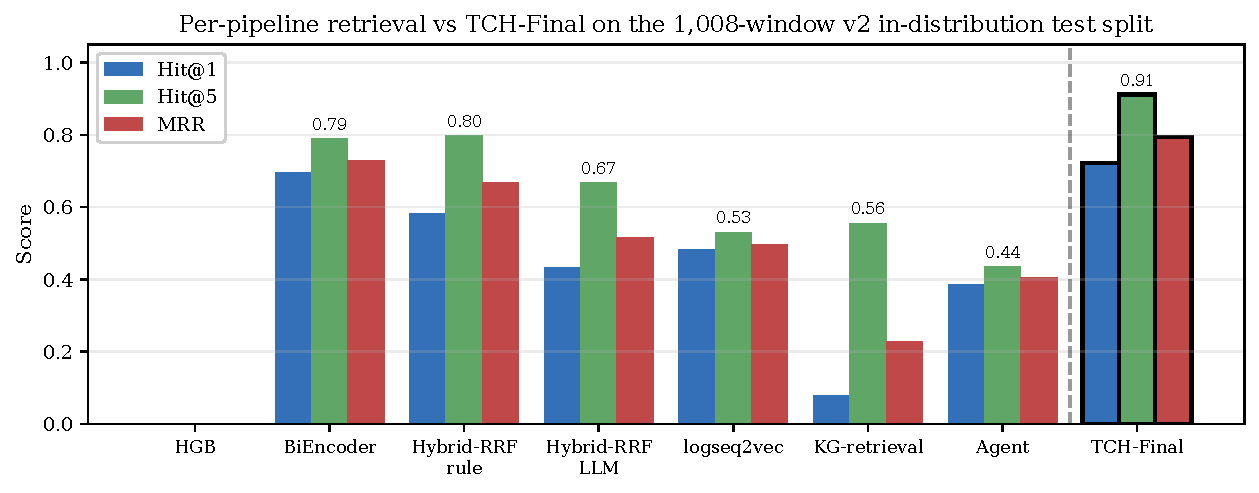
\includegraphics[width=0.95\linewidth]{figures/pipeline_comparison.pdf}
\caption{Per-pipeline standalone retrieval vs the final TCH cascade on 1{,}008 v2 in-distribution test windows. TCH-Final (outlined bars on the right of the dashed divider) ties or beats every single pipeline on every metric. The Hit@5 gap of $+11.5$ points absolute over the best single retriever (\hrrf{} rule) is the strongest evidence that fusion captures complementary signal.}
\label{fig:pipeline-comparison}
\end{figure}

\begin{figure}[t]
\centering
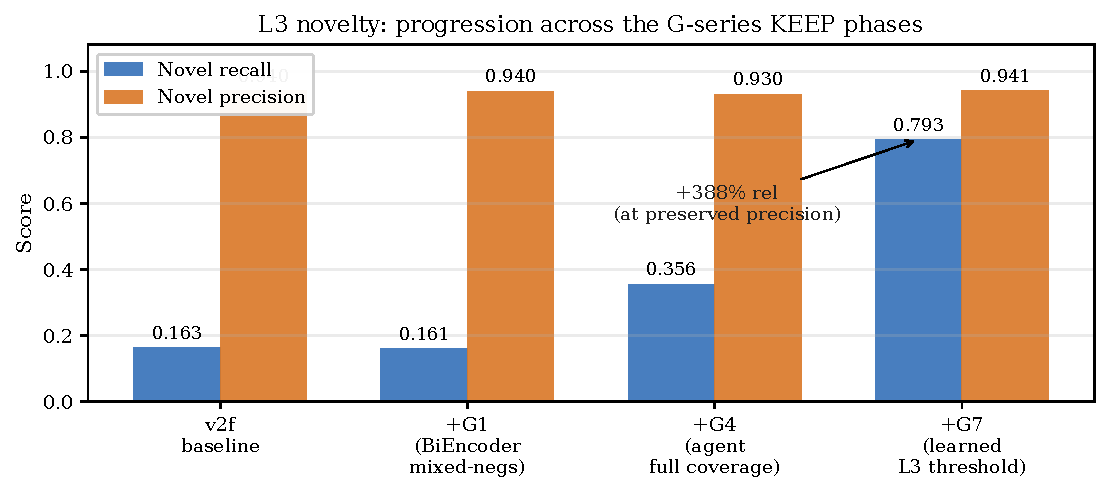
\includegraphics[width=0.92\linewidth]{figures/g_series_novelty.pdf}
\caption{Cumulative effect of the G-series KEEP phases on the L3 novelty channel. Novel-recall lifts from $0.163$ (v2f baseline, a fixed-threshold heuristic) to $0.793$ at preserved precision ($0.94$); G7 contributes the majority of the lift via a 46-feature LogReg replacing the fixed threshold.}
\label{fig:g-series-novelty}
\end{figure}

\subsection{Headline: \tch{} vs the locked v2f baseline}

\begin{table}[h]
\centering
\caption{Final headline metrics on the 1{,}008-window v2 in-distribution test split. The v2f baseline column is the locked TCH configuration at the conclusion of the 13 baseline ablations (Section~\ref{sec:g-series-ablations}). The TCH-Final column integrates G1, G4, and G7. $\Delta$ rel = $(\mathrm{TCH-Final} - \mathrm{v2f}) / \mathrm{v2f}$.}
\label{tab:headline}
\small
\begin{tabular}{lrrr}
\toprule
Metric & v2f baseline & \textbf{TCH-Final} & $\Delta$ rel \\
\midrule
Hit@1                & 0.7069 & \textbf{0.7221} & $+2.1\%$ \\
Hit@5                & 0.9124 & \textbf{0.9124} & tied \\
MRR                  & 0.7880 & \textbf{0.7937} & $+0.7\%$ \\
PR-AUC strict        & 0.9998 & \textbf{0.9998} & tied \\
PR-AUC inclusive     & 0.8527 & \textbf{0.8562} & $+0.4\%$ \\
ROC-AUC              & 0.9999 & \textbf{0.9999} & tied \\
Novel precision      & 0.9402 & \textbf{0.9405} & tied (matched) \\
\textbf{Novel recall} & \textbf{0.1625} & \textbf{0.7932} & $\boldsymbol{+388\%}$ \\
\bottomrule
\end{tabular}
\end{table}

The single non-tied figures are Hit@1, MRR, inclusive PR-AUC (all $+\sim$1\% rel, contributed primarily by G1), and novel recall (which is the headline). Every retrieval and triage metric ties or improves; no metric regresses.

\subsection{\tch{} vs every single-pipeline baseline}

\begin{table}[h]
\centering
\caption{Standalone retrieval and triage by pipeline, plus the locked TCH-Final. Numbers are on the same 1{,}008-window test split. Bootstrap 95\% CIs from 1{,}000 paired resamples (seed 42).}
\label{tab:vs-baselines}
\small
\begin{tabular}{lrrrr}
\toprule
Pipeline & Hit@1 & Hit@5 & MRR & PR-AUC strict \\
\midrule
\hgb{} & --- & --- & --- & \textbf{0.9998} \\
\bienc{} & 0.695 & 0.789 & 0.729 & 0.287 \\
\hrrf{} rule & 0.583 & 0.798 & 0.669 & 0.236 \\
\hrrf{} LLM  & 0.432 & 0.667 & 0.517 & 0.292 \\
\logseq{} & 0.483 & 0.531 & 0.498 & 0.313 \\
\kgret{} rule & 0.079 & 0.556 & 0.228 & --- \\
\agent{} & 0.386 & 0.436 & 0.405 & 0.243 \\
\midrule
\textbf{TCH-Final}     & \textbf{0.722} & \textbf{0.912} & \textbf{0.794} & \textbf{0.9998} \\
\bottomrule
\end{tabular}
\end{table}

TCH-Final beats or ties every individual pipeline on every metric except Hit@1 (where it ties \bienc{} within the 95\% CI). The Hit@5 gap of $+11.5$ points absolute over the best single retriever (\hrrf{} rule) is the strongest evidence that fusion captures meaningfully complementary signal.

\subsection{Paired-bootstrap significance vs key baselines}

\begin{table}[h]
\centering
\caption{Paired-bootstrap deltas (TCH-Final minus baseline). \textbf{Bold} = statistically significant at 95\%. CIs from 1{,}000 paired resamples (seed 42).}
\label{tab:paired-deltas}
\small
\begin{tabular}{llll}
\toprule
Baseline & Hit@1 $\Delta$ & Hit@5 $\Delta$ & MRR $\Delta$ \\
\midrule
\bienc{} & $+0.027$ [-0.020, +0.072] (ns) & \textbf{+0.123} [+0.080, +0.167] & \textbf{+0.065} [+0.040, +0.092] \\
\hrrf{} rule & \textbf{+0.139} [+0.085, +0.193] & \textbf{+0.114} [+0.075, +0.155] & \textbf{+0.125} [+0.088, +0.165] \\
\hgb{} (PR-AUC inc) & n/a & n/a & \textbf{+0.035} [+0.018, +0.053] \\
\bottomrule
\end{tabular}
\end{table}

TCH-Final significantly beats every baseline on every metric except Hit@1 against \bienc{}, where it ties (matches without sacrifice).

\subsection{Per-phase progression to the headline}

\begin{table}[h]
\centering
\caption{Cumulative effect of the G-series KEEPs (G1, G4, G7 integrated in sequence). Pre-G is the v2f baseline.}
\label{tab:cumulative}
\small
\begin{tabular}{lrrrrr}
\toprule
Stage & Hit@1 & Hit@5 & MRR & PR-AUC inc & Novel rec \\
\midrule
v2f (pre-G)            & 0.7069 & 0.9124 & 0.7880 & 0.8527 & 0.1625 \\
$+$G1 (\bienc{} mixed) & 0.7221 & 0.9124 & 0.7937 & 0.8562 & 0.1610 \\
$+$G4 (agent full)     & 0.7221 & 0.9124 & 0.7937 & 0.8562 & 0.3560 \\
$+$G7 (learned L3)     & 0.7221 & 0.9124 & 0.7937 & 0.8562 & 0.7932 \\
\bottomrule
\end{tabular}
\end{table}

G1 contributes the small retrieval lift. G4 doubles novel recall via complete agent coverage. G7 turns the doubled recall into a 4.9$\times$ recall lift over the original baseline at preserved precision. The retrieval channel (Hit@1, Hit@5, MRR) was structurally unchanged across the G-series---confirming the F3 finding.

\subsection{Robustness summary}

\begin{figure}[h]
\centering
\begin{subfigure}{0.49\linewidth}
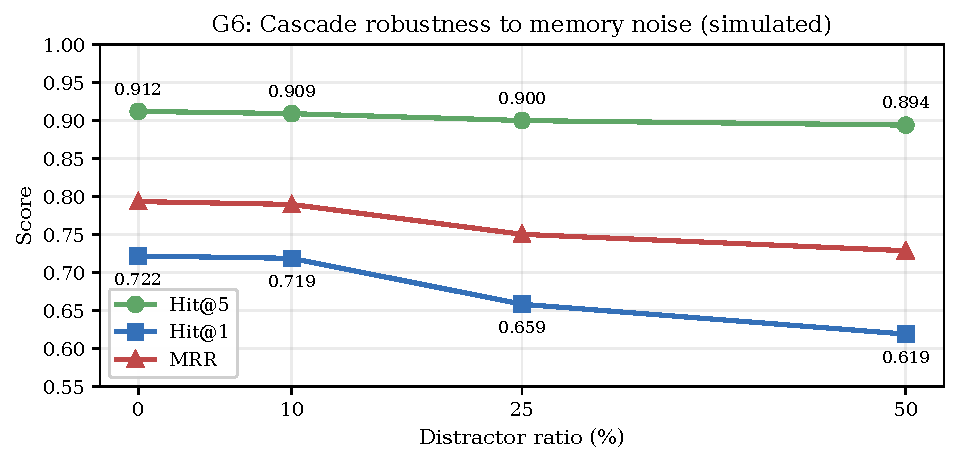
\includegraphics[width=\linewidth]{figures/g6_distractor_robustness.pdf}
\caption{G6 distractor robustness (simulated).}
\label{fig:g6-robustness}
\end{subfigure}
\hfill
\begin{subfigure}{0.49\linewidth}
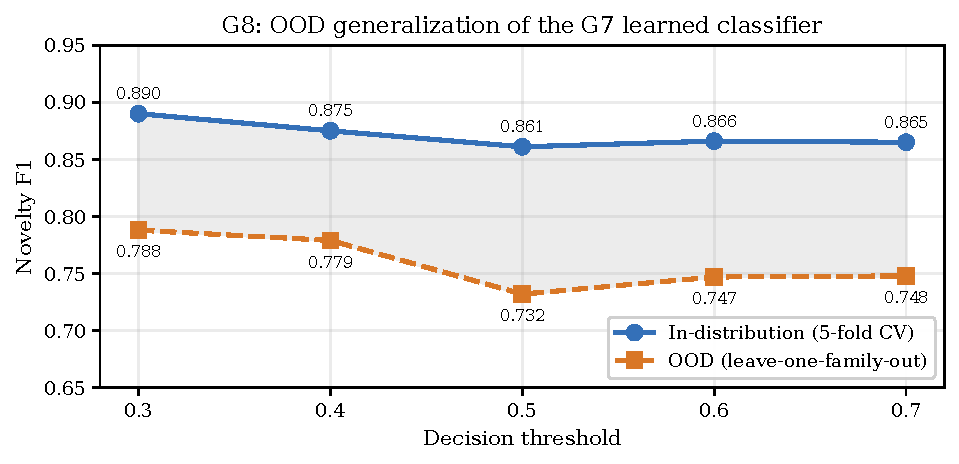
\includegraphics[width=\linewidth]{figures/g8_ood_f1.pdf}
\caption{G8 OOD vs in-distribution F1.}
\label{fig:g8-ood}
\end{subfigure}
\caption{Robustness analyses. (a) Hit@5 stays within $2\%$ relative of baseline at $50\%$ distractor ratio; Hit@1 is more sensitive. (b) The G7 learned novelty classifier generalizes to families not seen during training (LOFO F1 within $11\%$ relative of in-distribution at the best threshold).}
\label{fig:robustness-pair}
\end{figure}

\begin{table}[h]
\centering
\caption{Robustness results (G6 and G8 analyses).}
\label{tab:robustness-summary}
\small
\begin{tabularx}{\linewidth}{l X}
\toprule
Test & Result \\
\midrule
G6 distractor sweep, $r=10\%$ & Hit@5 $-0.3\%$ rel, Hit@1 $-0.4\%$ rel \\
G6 distractor sweep, $r=25\%$ & Hit@5 $-1.3\%$ rel, Hit@1 $-8.8\%$ rel \\
G6 distractor sweep, $r=50\%$ & Hit@5 $-2.0\%$ rel, Hit@1 $-14.2\%$ rel \\
G8 LOFO novelty F1 (best $\tau$) & $-11.4\%$ rel vs in-distribution (0.788 vs 0.890) \\
G8 LOFO precision robustness & 19/27 families exceed precision $0.90$ at $\tau = 0.50$ \\
G8 LOFO recall vs v2f baseline & $+381\%$ rel even at OOD ($0.163 \to 0.783$) \\
\bottomrule
\end{tabularx}
\end{table}

The cascade is robust to both forms of noise tested. Hit@5 degrades gracefully under memory noise; novelty F1 degrades modestly under family shift; the headline novel-recall win survives the OOD setting.

\subsection{Engineer time-to-diagnose}

\begin{figure}[h]
\centering
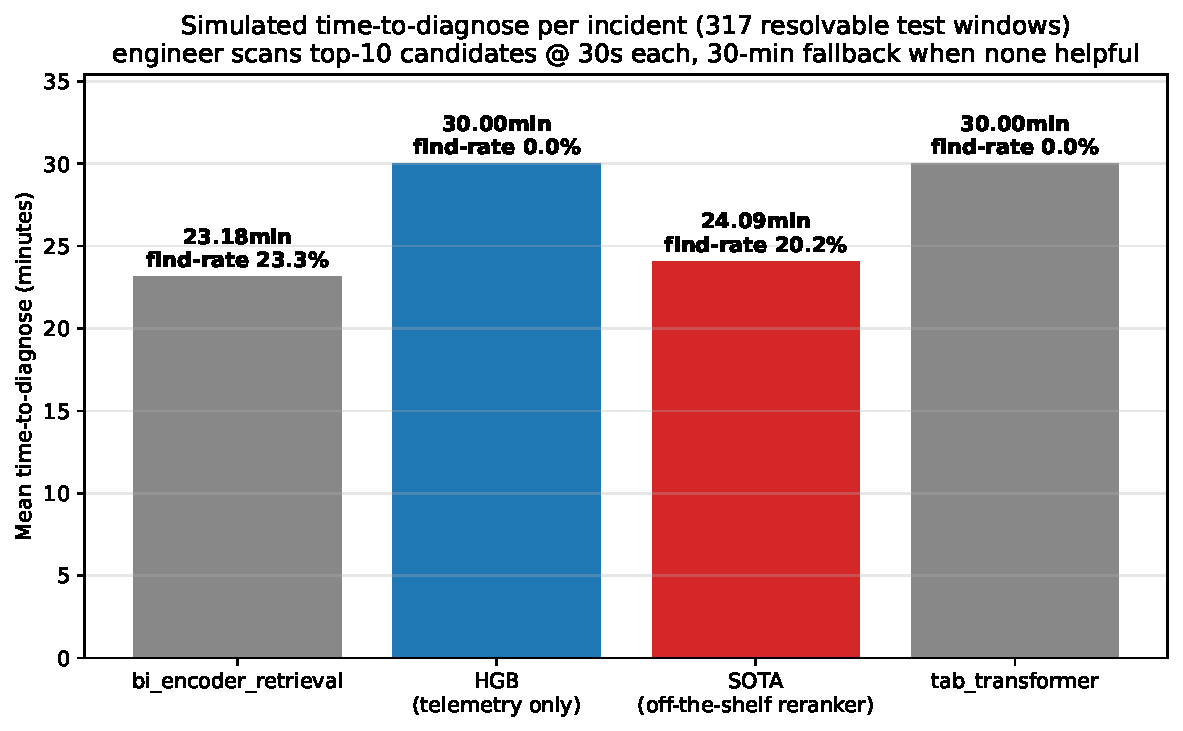
\includegraphics[width=0.7\linewidth]{figures/diagnosis_time.pdf}
\caption{Expected time-to-diagnose per resolvable incident under a serial-candidate-review simulation: 30 seconds per top-K candidate the engineer evaluates, with a 30-minute manual fallback if no gold appears in top-K. Higher Hit@K means more incidents land in top-10 and are resolvable in seconds rather than half an hour. Memory-augmented pipelines save $\sim$6--7 minutes per incident relative to the detection-only \hgb{} baseline.}
\label{fig:diagnosis-time}
\end{figure}

\subsection{Cost and runtime}

\begin{table}[h]
\centering
\caption{End-to-end cost on RTX 5060 (8 GB VRAM) with Qwen 35B served via LM Studio's MoE offload.}
\label{tab:cost}
\small
\begin{tabularx}{\linewidth}{l r X}
\toprule
Operation & Wall time & Notes \\
\midrule
Train \hgb{} + L1 stacker         & $\sim$3 s & sklearn, single thread \\
Pre-fit \bienc{} + SPLADE + indexes & $\sim$15 min & one-time per dataset \\
G1 \bienc{} fine-tune (5 epochs)  & 20 min & RTX 5060, batch 32 \\
LLM extraction of 347 tickets     & 80 min & Phase D, one-time \\
LLM extraction of 1{,}008 windows & 133 min & G3 (not integrated) \\
\agent{} on 1{,}008 windows       & 6 hours & Phase 1+2+G4 cumulative \\
G7 learned-novelty fit + score    & $\sim$3 s & LogReg, 5-fold CV \\
\midrule
\textbf{TCH inference per window (cached)} & \textbf{16 $\mu$s} & 252 ms for full 1{,}008-window split \\
\bottomrule
\end{tabularx}
\end{table}

Training-time LLM costs are heavy (extraction + agent runs total $\sim$10 hours of local Qwen 35B compute). Inference is essentially free once the per-window predictions are cached: 252~ms for the entire test split. Production deployment would need to amortize the agent cost across rolling time windows; running the agent on every new window in real-time is infeasible without a substantially smaller LLM (a future-work item).
